% Standalone compilable file for generating pipeline figures as PDFs
% Compile with: pdflatex figures_standalone.tex
% This will generate figures_standalone.pdf containing all figures

\documentclass[tikz, border=10pt]{standalone}
\usepackage{tikz}
\usetikzlibrary{shapes.geometric, arrows.meta, positioning, fit, backgrounds, calc}
\usepackage{amsmath}

\begin{document}

% ============================================================================
% FIGURE 1: Pipeline Architecture
% ============================================================================
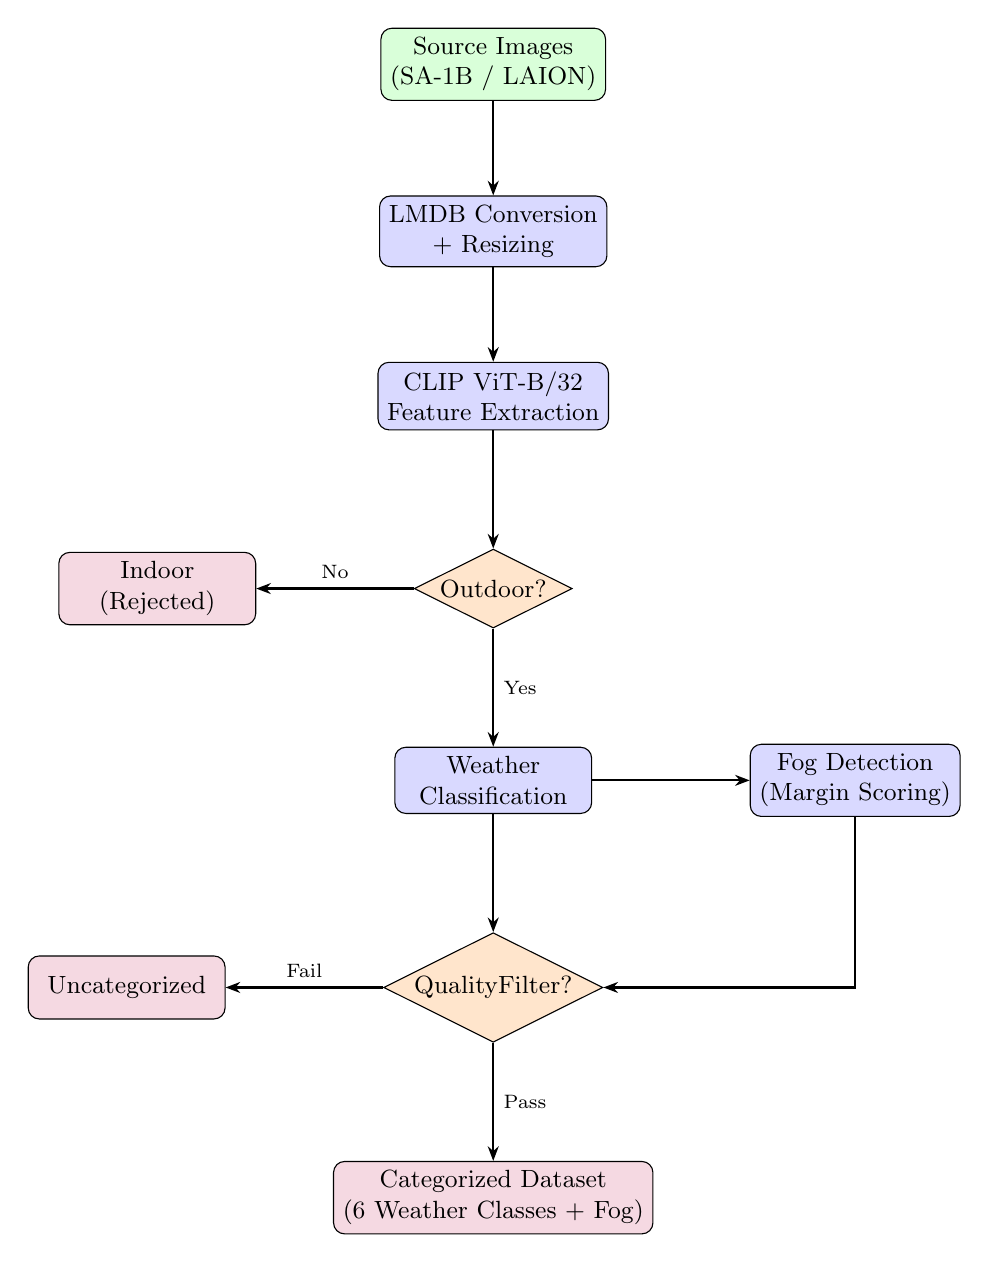
\begin{tikzpicture}[
    node distance=1.2cm and 1.5cm,
    box/.style={rectangle, draw, rounded corners, minimum width=2.5cm, minimum height=0.8cm, align=center, font=\small},
    process/.style={box, fill=blue!15},
    decision/.style={diamond, draw, aspect=2, fill=orange!20, font=\small, inner sep=1pt},
    data/.style={box, fill=green!15},
    output/.style={box, fill=purple!15},
    arrow/.style={-{Stealth[scale=0.8]}, thick}
]

% Input
\node[data] (input) {Source Images\\(SA-1B / LAION)};

% Preprocessing
\node[process, below=of input] (lmdb) {LMDB Conversion\\+ Resizing};

% CLIP Encoding
\node[process, below=of lmdb] (clip) {CLIP ViT-B/32\\Feature Extraction};

% Indoor/Outdoor Decision
\node[decision, below=1.5cm of clip] (io-decision) {Outdoor?};

% Indoor output
\node[output, left=2cm of io-decision] (indoor) {Indoor\\(Rejected)};

% Weather Classification
\node[process, below=1.5cm of io-decision] (weather) {Weather\\Classification};

% Fog Detection
\node[process, right=2cm of weather] (fog) {Fog Detection\\(Margin Scoring)};

% Quality Filter
\node[decision, below=1.5cm of weather] (quality) {Quality\\Filter?};

% Uncategorized
\node[output, left=2cm of quality] (uncat) {Uncategorized};

% Final Output
\node[output, below=1.5cm of quality] (output) {Categorized Dataset\\(6 Weather Classes + Fog)};

% Arrows
\draw[arrow] (input) -- (lmdb);
\draw[arrow] (lmdb) -- (clip);
\draw[arrow] (clip) -- (io-decision);
\draw[arrow] (io-decision) -- node[above, font=\scriptsize] {No} (indoor);
\draw[arrow] (io-decision) -- node[right, font=\scriptsize] {Yes} (weather);
\draw[arrow] (weather) -- (fog);
\draw[arrow] (fog) |- (quality);
\draw[arrow] (weather) -- (quality);
\draw[arrow] (quality) -- node[above, font=\scriptsize] {Fail} (uncat);
\draw[arrow] (quality) -- node[right, font=\scriptsize] {Pass} (output);

\end{tikzpicture}

\newpage

% ============================================================================
% FIGURE 2: Prompt Ensemble Scoring
% ============================================================================
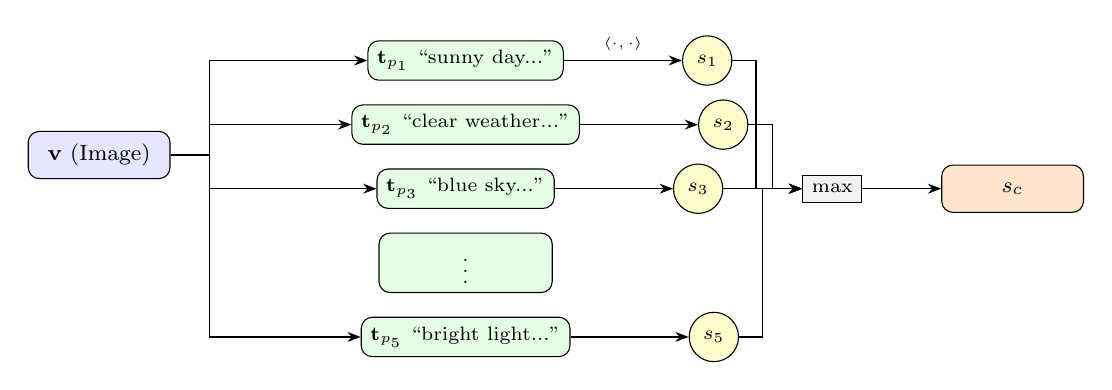
\begin{tikzpicture}[
    node distance=0.8cm,
    embed/.style={rectangle, draw, rounded corners, fill=blue!10, minimum width=1.8cm, minimum height=0.6cm, font=\footnotesize},
    prompt/.style={rectangle, draw, rounded corners, fill=green!10, minimum width=2.2cm, minimum height=0.5cm, font=\scriptsize},
    score/.style={circle, draw, fill=yellow!20, minimum size=0.6cm, font=\scriptsize},
    op/.style={rectangle, draw, fill=gray!10, font=\scriptsize}
]

% Image embedding
\node[embed] (img) {$\mathbf{v}$ (Image)};

% Prompt embeddings
\node[prompt, right=2.5cm of img, yshift=1.2cm] (p1) {$\mathbf{t}_{p_1}$ ``sunny day...''};
\node[prompt, below=0.3cm of p1] (p2) {$\mathbf{t}_{p_2}$ ``clear weather...''};
\node[prompt, below=0.3cm of p2] (p3) {$\mathbf{t}_{p_3}$ ``blue sky...''};
\node[prompt, below=0.3cm of p3] (p4) {$\vdots$};
\node[prompt, below=0.3cm of p4] (p5) {$\mathbf{t}_{p_5}$ ``bright light...''};

% Similarity scores
\node[score, right=1.5cm of p1] (s1) {$s_1$};
\node[score, right=1.5cm of p2] (s2) {$s_2$};
\node[score, right=1.5cm of p3] (s3) {$s_3$};
\node[score, right=1.5cm of p5] (s5) {$s_5$};

% Max operation
\node[op, right=1cm of s3] (max) {$\max$};

% Final score
\node[embed, right=1cm of max, fill=orange!20] (final) {$s_c$};

% Arrows
\draw[-{Stealth}] (img.east) -- ++(0.5,0) |- (p1.west);
\draw[-{Stealth}] (img.east) -- ++(0.5,0) |- (p2.west);
\draw[-{Stealth}] (img.east) -- ++(0.5,0) |- (p3.west);
\draw[-{Stealth}] (img.east) -- ++(0.5,0) |- (p5.west);

\draw[-{Stealth}] (p1) -- node[above, font=\tiny] {$\langle\cdot,\cdot\rangle$} (s1);
\draw[-{Stealth}] (p2) -- (s2);
\draw[-{Stealth}] (p3) -- (s3);
\draw[-{Stealth}] (p5) -- (s5);

\draw[-{Stealth}] (s1.east) -- ++(0.3,0) |- (max.west);
\draw[-{Stealth}] (s2.east) -- ++(0.3,0) |- (max.west);
\draw[-{Stealth}] (s3) -- (max);
\draw[-{Stealth}] (s5.east) -- ++(0.3,0) |- (max.west);

\draw[-{Stealth}] (max) -- (final);

\end{tikzpicture}

\newpage

% ============================================================================
% FIGURE 3: Fog Detection Margin Scoring (NEW)
% ============================================================================
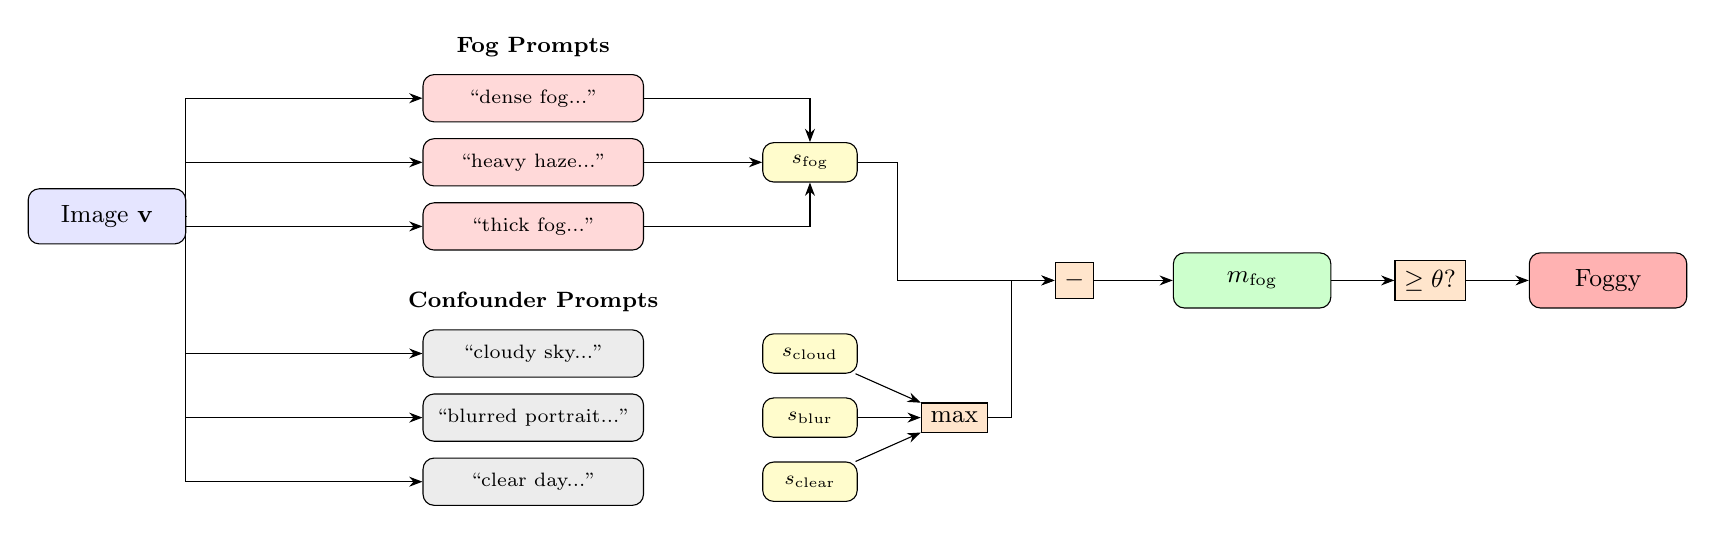
\begin{tikzpicture}[
    node distance=1cm,
    embed/.style={rectangle, draw, rounded corners, fill=blue!10, minimum width=2cm, minimum height=0.7cm, font=\small, align=center},
    prompt/.style={rectangle, draw, rounded corners, minimum width=2.8cm, minimum height=0.6cm, font=\scriptsize, align=center},
    fog/.style={prompt, fill=red!15},
    conf/.style={prompt, fill=gray!15},
    score/.style={rectangle, draw, rounded corners, fill=yellow!20, minimum width=1.2cm, minimum height=0.5cm, font=\scriptsize},
    op/.style={rectangle, draw, fill=orange!20, font=\small},
    result/.style={rectangle, draw, rounded corners, fill=green!20, minimum width=2cm, minimum height=0.7cm, font=\small}
]

% Image
\node[embed] (img) {Image $\mathbf{v}$};

% Fog prompts
\node[fog, right=3cm of img, yshift=1.5cm] (fog1) {``dense fog...''};
\node[fog, below=0.2cm of fog1] (fog2) {``heavy haze...''};
\node[fog, below=0.2cm of fog2] (fog3) {``thick fog...''};

% Fog score
\node[score, right=1.5cm of fog2] (sfog) {$s_{\text{fog}}$};

% Confounder prompts
\node[conf, below=1cm of fog3] (cloud) {``cloudy sky...''};
\node[conf, below=0.2cm of cloud] (blur) {``blurred portrait...''};
\node[conf, below=0.2cm of blur] (clear) {``clear day...''};

% Confounder scores
\node[score, right=1.5cm of cloud] (scloud) {$s_{\text{cloud}}$};
\node[score, right=1.5cm of blur] (sblur) {$s_{\text{blur}}$};
\node[score, right=1.5cm of clear] (sclear) {$s_{\text{clear}}$};

% Max confounder
\node[op, right=0.8cm of sblur] (maxconf) {$\max$};

% Margin calculation
\node[op, right=2.5cm of sfog, yshift=-1.5cm] (minus) {$-$};

% Final margin
\node[result, right=1cm of minus] (margin) {$m_{\text{fog}}$};

% Threshold decision
\node[op, right=0.8cm of margin] (thresh) {$\geq \theta$?};

% Result
\node[result, right=0.8cm of thresh, fill=red!30] (foggy) {Foggy};

% Arrows
\draw[-{Stealth}] (img) -- ++(1,0) |- (fog1.west);
\draw[-{Stealth}] (img) -- ++(1,0) |- (fog2.west);
\draw[-{Stealth}] (img) -- ++(1,0) |- (fog3.west);
\draw[-{Stealth}] (img) -- ++(1,0) |- (cloud.west);
\draw[-{Stealth}] (img) -- ++(1,0) |- (blur.west);
\draw[-{Stealth}] (img) -- ++(1,0) |- (clear.west);

\draw[-{Stealth}] (fog1.east) -| (sfog);
\draw[-{Stealth}] (fog2) -- (sfog);
\draw[-{Stealth}] (fog3.east) -| (sfog);

\draw[-{Stealth}] (scloud) -- (maxconf);
\draw[-{Stealth}] (sblur) -- (maxconf);
\draw[-{Stealth}] (sclear) -- (maxconf);

\draw[-{Stealth}] (sfog.east) -- ++(0.5,0) |- (minus.west);
\draw[-{Stealth}] (maxconf.east) -- ++(0.3,0) |- (minus.west);

\draw[-{Stealth}] (minus) -- (margin);
\draw[-{Stealth}] (margin) -- (thresh);
\draw[-{Stealth}] (thresh) -- (foggy);

% Labels
\node[above=0.1cm of fog1, font=\footnotesize\bfseries] {Fog Prompts};
\node[above=0.1cm of cloud, font=\footnotesize\bfseries] {Confounder Prompts};

\end{tikzpicture}

\end{document}
